% filepath: /home/balogh/code/tp1/CoP-DDAHC-pages/docs/document_processing_pipeline.tex
\documentclass[12pt,a4paper]{article}
\usepackage[utf8]{inputenc}
\usepackage[slovak]{babel}
\usepackage{hyperref}
\usepackage{enumitem}
\usepackage{geometry}
\geometry{margin=2.5cm}

\title{Spracovanie dokumentov}
\author{}
\date{}

\begin{document}

\maketitle

Celá pipeline spracovania dokumentov pozostáva z niekoľkých fáz. Sú zobrazené na diagrame na obr. \ref{fig:pipeline_diagram}.

\begin{figure}[h]
    \centering
    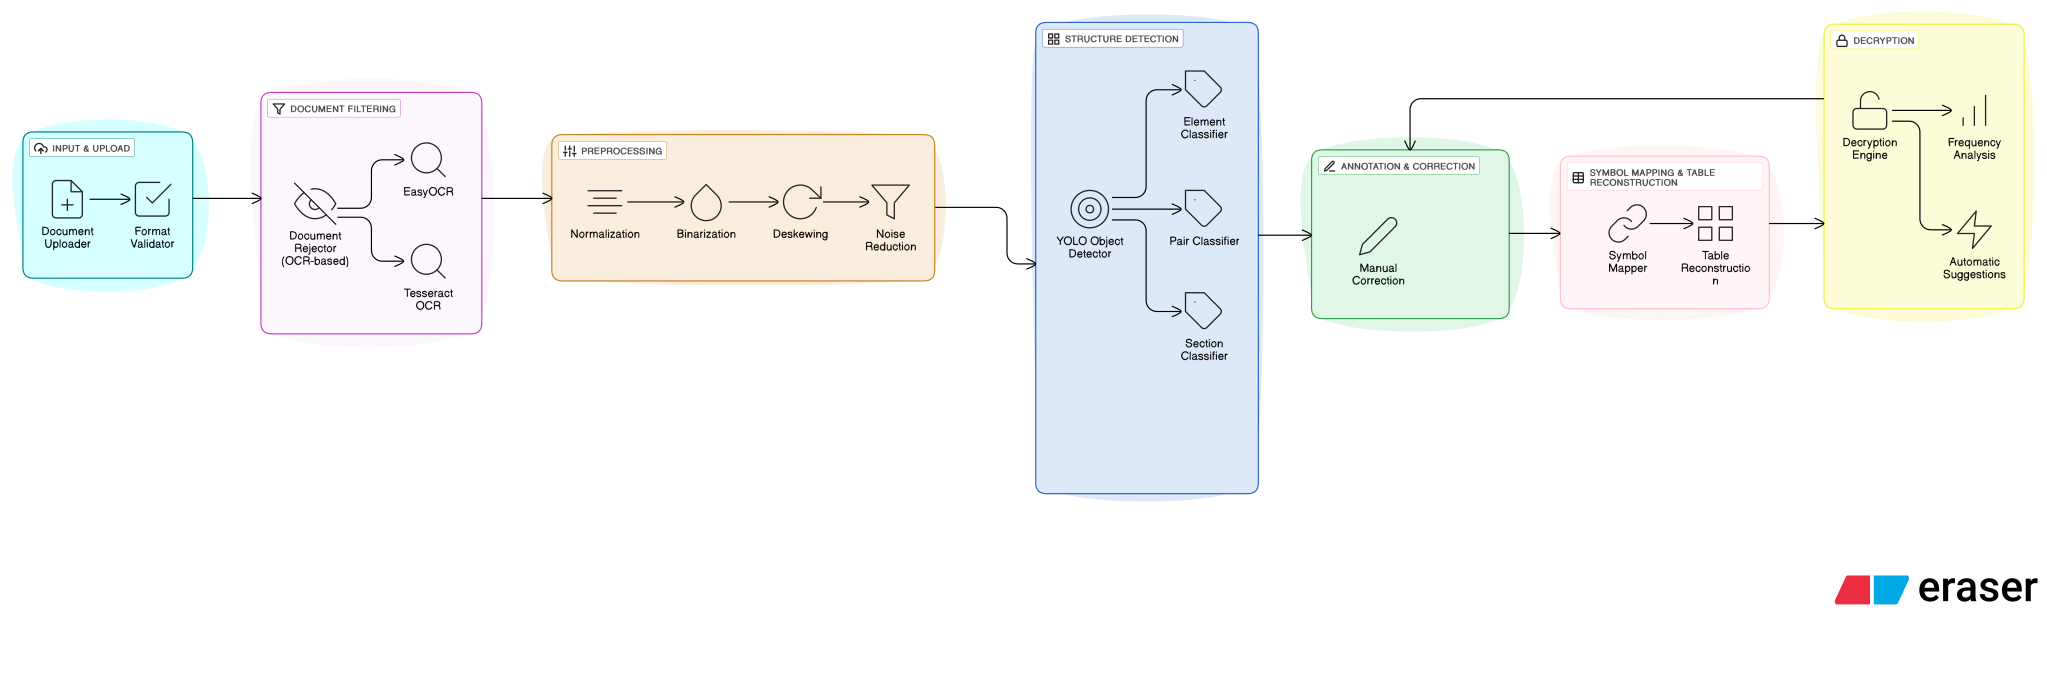
\includegraphics[width=0.8\textwidth]{doc/img/pipeline_diagram.png}
    \caption{Diagram spracovania dokumentov}
    \label{fig:pipeline_diagram}
\end{figure}

\section{Úvodná kontrola (document rejector)}

Po nahraní nového obrázka systém najprv vyhodnocuje, či ide o historický dokument, alebo o nesúvisiaci obrázok (napríklad fotografia auta, zvieraťa a podobne). Cieľom je zabrániť spracovaniu irelevantných obrázkov.

Na tento účel využívame OCR (optické rozpoznávanie znakov). Zo vstupného obrázka sa extrahujú slová. Ak sa podarí rozpoznať aspoň určitý počet slov (podľa nastaveného prahu), obrázok je prijatý na ďalšie spracovanie ako dokument. V opačnom prípade je odmietnutý. Týmto spôsobom sa automaticky filtrujú obrázky bez textu, ktoré pravdepodobne nepredstavujú historické dokumenty určené na ďalšie spracovanie.

V rámci experimentov bol najprv použitý \textbf{EasyOCR}~\cite{easyocr}, ktorý je lightweight, má podporu pre veľa jazykov, má dobrú výkonnosť a funguje dobre aj na iných obrázkoch ako čierny text na bielom pozadí. Fungoval dobre aj na písanom texte na historických dokumentoch. Ďalšou jeho výhodou bolo to, že čítal text postupne a pomocou parametra sa dal nastaviť maximálny počet textových boxov, ktoré sa mali rozpoznávať, čo značne urýchľovalo proces rozpoznávania. Tento parameter bol nastavený na rovnaké číslo ako threshold pre prijatie dokumentu. Experimentovaním s dokumentami a inými obrázkami sme dospeli k číslu 30 textových boxov ako optimálnej hodnote pre náš usecase. Toto číslo malo 100\% acceptance rate pre dokumenty a zároveň efektívne odmietalo obrázky, kde neboli dokumenty, ale napríklad zo značiek prečítal nejaké texty.

EasyOCR však spôsoboval viaceré problémy:
\begin{itemize}
    \item prvotné načítanie knižnice bolo pomalé (2-3 sekundy),
    \item vyžadoval veľké množstvo závislostí, čo značne predlžovalo čas potrebný na zostavenie docker image (viac ako 10 minút),
    \item výsledný docker image mal veľkú veľkosť (až 17 GB).
\end{itemize}

Z týchto dôvodov sme ho nahradili za \textbf{Tesseract OCR}~\cite{tesseract}. Tesseract OCR je jeden z najpoužívanejších OCR nástrojov, je open-source a dosahuje vysokú presnosť rozpoznávania textu. Tiež má podporu pre veľa jazykov a zároveň podporu pre písaný text. Taktiež existuje Python API pre Tesseract (\textbf{pytesseract}~\cite{pytesseract}), čo umožňuje jednoduché integrovanie do nášho systému.

Tesseract sa sťahuje už ako skompilovaný binárny súbor, čo znamená, že nie je potrebné buildnuť toľko dependencies ako pri EasyOCR. Vďaka tomu sa čas buildnutia docker image znížil z viac ako 10 minút na približne 20 sekúnd a veľkosť docker image sa zmenšila z 17 GB na približne 2 GB. Prvé načítanie Tesseract knižnice trvá okolo 0.5 sekundy, čo je tiež značne zrýchlenie oproti EasyOCR a užívateľsky prívetivé.

Tesseract neumožňuje čítanie textu postupne a obrázky s veľkým množstvom textu zaberali dlhú dobu. Preto sa na zrýchlenie najprv zmenší obrázok a následne sa aplikuje sliding window mechanizmus. Pri tomto postupe sa obrázok skenuje po častiach a priebežne sa kumuluje počet rozpoznaných znakov. Ak počet rozpoznaných znakov prekročí nastavený limit, dokument je akceptovaný a prestáva sa ďalšie spracovanie.

Inferencia Tesseract OCR je vďaka skompilovanému binárnemu súboru rýchlejšia ako u EasyOCR, a preto celkový čas na vyhodnotenie dokumentu klesol o pár desatín sekundy pri zachovaní rovnakej presnosti detekcie na našich testovacích dokumentoch. Čas inferencie je momentálne v rozpätí okolo 0.25 až 0.5 sekundy na dokument.

\begin{figure}[h]
    \centering
    \includegraphics[width=0.45\textwidth]{doc/img/document_acceptor.png}
    \includegraphics[width=0.45\textwidth]{doc/img/document_rejector.png}
    \caption{Príklady akceptovaného a odmietnutého dokumentu pomocou Tesseract OCR.}
    \label{fig:document_rejector}
\end{figure}
Tesseract OCR nasiel 30 slov na lavom obrazku, tym sa sliding window mechanizmus zastavil a dokument bol akceptovany. Na obrazku vpravo Tesseract nasiel len 9 slov a sliding window algoritmus skoncil, takze dokument bol odmietnuty.
Vlavo: Historicky dokument
Vpravo: Obrázok č. 206391 z COCO datasetu \cite{coco} (dostupný na: http://cocodataset.org/#explore?id=206391).


\section{Predspracovanie obrázkov}

Po úspešnom prijatí dokumentu nasleduje fáza predspracovania obrázkov. Cieľom tejto fázy je zlepšiť kvalitu obrázkov a pripraviť ich na následné kroky spracovania, ako je detekcia a klasifikácia elementov. Predspracovanie zahŕňa niekoľko krokov, vrátane:

\section{Detekcia a klasifikácia elementov, párov a sekcií}

Po úvodnom filtrovaní dokumentov nasleduje kľúčová fáza spracovania – extrakcia štruktúry a obsahu z kľúčových dokumentov (cipher keys). Tieto dokumenty majú špecifickú hierarchickú štruktúru: skladajú sa zo sekcií (napr. tabuľky), ktoré obsahujú páry (dvojice znakov otvorený text – šifra) a tie sú tvorené samotnými elementmi (jednotlivé symboly).

Na túto úlohu sme zvolili architektúru \textbf{YOLO} (You Only Look Once), konkrétne verziu \textbf{YOLOv11}, ktorá predstavuje aktuálny state-of-the-art v oblasti detekcie objektov v reálnom čase.

\subsection{Príprava dát a datasetov}

Pre trénovanie modelov sme museli pripraviť dva hlavné datasety. Prvým bol \textbf{IAM Handwriting Database}~\cite{iam_database}, ktorý obsahuje veľké množstvo anotovaného rukou písaného textu. Tento dataset slúžil primárne na predtrénovanie modelov (transfer learning), aby sa neurónová sieť naučila rozpoznávať črty rukopisu skôr, než začne riešiť špecifickú úlohu šifier. Pôvodné XML anotácie sme pomocou skriptov konvertovali do formátu YOLO.

Druhým datasetom bol dataset \textbf{Transcendino} poskytnutý naším vedúcim, ktorý obsahuje historické šifrovacie kľúče. K tvorbe tohto datasetu sme v rámci tímového projektu prispeli aj my anotovaním dokumentov. Tieto dokumenty boli manuálne anotované pomocou nástroja \textbf{LabelMe}~\cite{labelme}, kde sme vyznačovali bounding boxy pre elementy, páry a sekcie. Následne sme vytvorili konverzný skript, ktorý transformoval JSON výstupy z LabelMe do YOLO formátu a rozdelil dáta na trénovaciu, validačnú a testovaciu množinu v pomere 70:20:10.

\subsection{Experimentálne stratégie trénovania}

Keďže detekcia vnorených objektov (element je v páre, pár je v sekcii) je pre štandardné detektory náročná, navrhli a porovnali sme v rámci súboru \texttt{training\_grid.py} šesť rôznych trénovacích stratégií:

\begin{enumerate}[label=\Alph*.]
    \item \textbf{Multiclass}: Trénovanie jedného modelu, ktorý sa snaží detegovať všetky tri triedy (element, pár, sekcia) naraz.
    \item \textbf{IAM Pretraining + Multiclass}: Rovnaký prístup ako A, ale model bol najprv predtrénovaný na IAM datasete.
    \item \textbf{Single Class}: Trénovanie troch samostatných modelov – jeden špecializovaný čisto na elementy, druhý na páry a tretí na sekcie.
    \item \textbf{IAM Pretraining + Single Class}: Samostatné modely predtrénované na IAM datasete.
    \item \textbf{Hierarchické trénovanie}: Inovatívny prístup inšpirovaný curriculum learningom. Najprv sa natrénuje model na najmenších objektoch (elementoch). Váhy tohto modelu sa použijú ako základ pre trénovanie modelu na pároch a ten následne slúži ako základ pre model na sekcie. Týmto sa sieť učí skladať zložitejšie štruktúry z jednoduchších.
    \item \textbf{IAM Pretraining + Hierarchické trénovanie}: Kombinácia predtrénovania na rukopise a hierarchického prístupu.
\end{enumerate}

\subsection{Výsledky}

Experimenty ukázali, že pre naše potreby je najvhodnejší hierarchický prístup kombinovaný s predtrénovaním na IAM datasete (Stratégia F). Štandardný Multiclass prístup mal problémy s prekrývajúcimi sa bounding boxmi (keďže pár obklopuje elementy), čo viedlo k nižšej presnosti. Hierarchický prístup umožnil modelu lepšie pochopiť kontext a vzťahy medzi objektmi. Použitie modelu YOLOv11 vo veľkosti \texttt{x} (extra large) zabezpečilo dostatočnú kapacitu siete na zachytenie jemných detailov historického rukopisu.

\subsection{Integrácia do produkčného prostredia}

Keďže spracovanie má byť len poloautomatické a anotácie navrhnuté naším nástrojom môže človek potom opraviť, na implementáciu sme zvolili menší model \texttt{_____}, keďže dosahuje stále výbornú presnosť a zároveň je rýchly na inferenciu a menej náročný na zdroje.

\section*{Použité zdroje}

\begingroup
\renewcommand{\section}[2]{}%
\begin{thebibliography}{9}

\bibitem{easyocr}
JaidedAI,
\textit{EasyOCR},
2024, verzia 1.7.2,
\url{https://github.com/JaidedAI/EasyOCR},
Dostupné z: \url{https://github.com/JaidedAI/EasyOCR} [cit. 2026-01-01]

\bibitem{tesseract}
Ray Smith, Stefan Weil, Zdenko Podobny a prispievatelia,
\textit{Tesseract OCR},
2024, verzia 4.1.3,
\url{https://github.com/tesseract-ocr/tesseract},
Dostupné z: \url{https://github.com/tesseract-ocr/tesseract} [cit. 2026-01-01]

\bibitem{pytesseract}
Samuel Hoffstaetter a prispievatelia,
\textit{pytesseract: Python-tesseract},
2024, verzia 0.3.10,
\url{https://github.com/madmaze/pytesseract},
Dostupné z: \url{https://github.com/madmaze/pytesseract} [cit. 2026-01-01]

\bibitem{iam_database}
Urs-Viktor Marti, Horst Bunke,
\textit{The IAM-database: An English Sentence Database for Off-line Handwriting Recognition},
International Journal on Document Analysis and Recognition,
vol. 5, č. 1, s. 39--46, 2002, Springer

\bibitem{labelme}
Kentaro Wada,
\textit{labelme: Image Polygonal Annotation with Python},
2018, GitHub repository,
\url{https://github.com/wkentaro/labelme}


@inproceedings{coco,
  title = {Microsoft COCO: Common Objects in Context},
  author = {Lin, Tsung-Yi and Maire, Michael and Belongie, Serge and Hays, James and Perona, Pietro and Ramanan, Deva and Dollár, Piotr and Zitnick, C. Lawrence},
  booktitle = {European Conference on Computer Vision (ECCV)},
  pages = {740--755},
  year = {2014},
  publisher = {Springer}
}

\end{thebibliography}
\endgroup

\end{document}
